\chapter{Polytopes}

This chapter will provide relevant background material in the theory of convex polytopes.  Proofs of any theorems which appear can be found in \cite{McMullenBook} (unless otherwise noted).

  The set \(\seta{1,2\dc n}\) will be denoted \(\brac n\).  Throughout, \(\R d\) will denote the real inner product space of column vectors of length \(d\) with real entries and the Euclidean inner product.  The set of vectors \(\setb{\ve e_i}{i\in\brac d}\sbset\R d\) is called the \dfn{standard basis} and \(\ve e_i\) has \(j\)th entry \((\ve e_i)_j=\begin{cases}0&\text{if }i\ne j\\ 1&\text{if }i=j\end{cases}\).  The vectors \(\ve 0_d, \ve 1_d\in\R d\) have \(j\)th entry \((\ve 0)_j=0\), and \((\ve 1)_j=1\) respectively.  When no confusion may arise, these vectors shall be denoted simply \(\ve 0\) and \(\ve 1\).  If \(\ve x, \ve y\in\R n\), then \(\ip{\ve x}{\ve y}\) will denote the inner product of \(\ve x\) and \(\ve y\), \(\norm{\ve x}=\ip{\ve x}{\ve x}^{1/2}\) is the Euclidean norm, and \(\B\eps{\ve x}=\setb{\ve y}{\norm{\ve x-\ve y}\le\eps}\) is the closed ball of radius \(\eps>0\) centered at \(\ve x\). No distinction shall be made between the vector space \(\R d\) and its dual \((\R d)^\ast\).  Therefore all vectors will be considered to be column vectors.  If \(A\sbset\RR\) and \(d\in\N\), then \(A^d=\setb{\ve x\in\R d}{\ip{\ve x}{\ve e_i}\in A\text{ for all }i\in\brac d}\).

\section{Hulls; or, The Parts That Touch the Water}

If \(\seta{\ve x_1,\ve x_2\dc \ve x_k}\sbset \R n\), then a vector \(\ve v\) is an \dfn{affine combination} of \(\ve x_1,\ve x_2\dc \ve x_k\) if there are elements \(\la_i\in\RR\) such that \(\ve v = \sum_{i\in\brac k}\la_i\ve x_i\) and \(\sum_{i\in\brac k}\la_i=1\).  If \(A\sbset \R n\), then the \dfn{affine hull} of \(A\) is the set\footnote{Note, in this definition (as well as that of the convex hull), \(A\) need not be a finite set.}
    \[
        \aff(A)
            =\setb{\sum_{i\in\brac k}\la_i\ve x_i}{\ve x_i\in A,\,\la_i\in \RR\text{ and }\sum_{i\in\brac k}\la_i=1}.
    \]

A set which is closed under taking affine combinations of its elements (that is, \(\aff(A)=A\)) is called an \dfn{affine set}.  The intersection of a family of affine sets is again an affine set.  Every affine subset of \(\R n\) is a translation of a linear subspace of \(\R n\).  If \(A\) is an affine set, and \(L\) is a linear subspace of \(\R n\) such that \(A=L+\ve b\), then the \dfn{dimension} of \(A\) is \(\dim A=\dim L\).  For example: \(\dim\mt=-1\); \(\dim\seta{\ve x}=0\); and \(\dim\aff\seta{\ve x,\ve y}=1\) for \(\ve x\ne\ve y\).

A set \(K\sbset \R n\) is \dfn{convex} if for each \(\ve x, \ve y\in K\) the set \(\setb{\la\ve x+(1-\la)\ve y}{0\le\la\le1}\sbset K\).  If \(\seta{\ve x_1,\ve x_2\dc \ve x_k}\sbset \R n\), then a vector \(\ve v\) is a \dfn{convex combination} of \(\ve x_1,\ve x_2\dc \ve x_k\) if there are elements \(\la_i\in\RR\) such that \(\ve v = \sum_{i\in\brac k}\la_i\ve x_i\), with \(\la_i\ge0\) and \(\sum_{i\in\brac k}\la_i=1\).  If \(A\sbset\R n\), then the \dfn{convex hull} of \(A\) is the set
    \[
        \conv(A)
            =\setb{\sum_{i\in\brac k}\la_i\ve x_i}{\ve x_i\in A,\,\la_i\ge0\text{ and }\sum_{i\in\brac k}\la_i=1}.
    \]
If \(K\) is convex, then \(\conv K=K\).  For each set \(A\), \(\conv A\sbset\aff A\).  The intersection of a family of convex sets is again a convex set.  The \dfn{dimension} of a convex set \(K\) is the dimension of its affine hull, \(\dim K=\dim\aff K\).

Both \(\aff\) and \(\conv\) are closure operators, that is:
    \begin{itemize}
        \item   \(A\sbset\aff A\) and \(A\sbset\conv A\);
        \item   if \(A\sbset B\), then \(\aff A\sbset\aff B\) and \(\conv A\sbset \conv B\); and
        \item\(\aff(\aff A)=\aff A\) and \(\conv(\conv A)=\conv A\).
    \end{itemize}
Both \(\aff A\) and \(\conv A\) are minimal in the sense that \(\aff A\) is the intersection of all affine sets which contain \(A\), and \(\conv A\) is the intersection of all convex sets which contain \(A\).

If \(H\sbset\R n\) is an affine set with \(\dim H=n-1\), then \(H\) is called a \dfn{hyperplane}, and there is a pair \((\ve\xi,t)\) such that \(\ve\xi\in\R n\) with \(\ip{\ve\xi}{\ve\xi}=1\) and \(t\in\RR\) with \(H=\setb{\ve x\in\R n}{\ip{\ve\xi}{\ve x}=t}\) (here, \(\ve\xi\) is not unique unless \(n=0\) (if \(n\ne0\), then there are exactly two such vectors, and the other one is \(-\ve\xi\))).  The pair \((H, \ve\xi)\) is called an \dfn{oriented hyperplane}, and the \dfn{positive} and \dfn{negative closed halfspaces} of \(H\) are defined by, respectively, \(H^+=\setb{\ve x\in\R n}{\ip{\ve\xi}{\ve x}\ge t}\) and \(H^-=\setb{\ve\xi\in\R n}{\ip{\ve\xi}{\ve x}\le t}\).  Thus \(H=H^+\cap H^-\).  The \dfn{positive} and \dfn{negative} \dfn{open half-spaces} \(H^{(+)}\) and \(H^{(-)}\) are defined by making the defining inequalities strict.  Alternatively, \(H^{(+)}=H^+\setminus H\) and \(H^{(-)}=H^-\setminus H\) .  A set of the form \(H^+\) or \(H^-\) is called a \dfn{closed half-space}.

\section{Polytopes (not `Galeorhinus Galeus')}

In this section convex polytopes\footnote{Throughout, all polytopes will be convex so the adjective ``convex'' shall be omitted.} will be defined in two different ways.  The proof of equivalence of these two definitions can be found in \cite{BronstedBook}, \cite{GrunBook}, \cite{McMullenBook} or \cite{ZieglerBook}.

An \dfn{\(\mathpzc H\)-polytope} is a bounded set of the form \(P=\bigcap\scr H\) where
    \[
        \scr H=\seta{H_1^+, H_2^+\dc H_k^+, H_{k+1}^-,H_{k+2}^-\dc H_\ell^-}
    \]
is a finite collection of closed halfspaces.  A \dfn{\(\mathpzc V\)-polytope} is the convex hull of a finite set of points in some Euclidean space \(\R k\).  A set \(P\) is  an \(\mathpzc H\)-polytope if and only if it is a \(\mathpzc V\)-polytope.  Henceforth the prefix will be omitted, and \(P\) shall be called a polytope.  If \(P\) is a polytope, then the set \(\vrt P\) is the (unique) minimal (under inclusion) set such that \(P=\conv(\vrt P)\).

The dimension of a polytope is its dimension as a convex set.  A polytope of dimension \(d\) is called a \dfn{\(d\)-polytope}.  If \(P\) is a \(d\)-polytope, then  a hyperplane \(H\) is called a \dfn{supporting hyperplane} of \(P\) if \(P\cap H\ne\mt\) and either \(P\sbset H^+\) or \(P\sbset H^-\).  A \dfn{face} of a polytope \(P\) is a subset \(F\) of \(P\) such that one of the following holds:
    \begin{enumerate}
        \item   \(F=\mt\); or
        \item   there is some supporting hyperplane \(H\) of \(P\) with \(F=H\cap P\); or
        \item   \(F=P\).
    \end{enumerate}
If \(F\) is a face of a polytope \(P\), then \(F\) is itself a polytope since \(F=\conv(F\cap\vrt P)\), further \(\vrt F=F\cap\vrt P\).  If \(\dim F=r\), then \(F\) is called an \dfn{\(r\)-face} of \(P\).  A face of a face of a polytope is again a face of the polytope.  A face of a polytope is called \dfn{proper} if it is neither empty, nor the whole polytope.  If \(P\) is a \(d\)-polytope, then a face of dimension
    \begin{itemize}
        \item   \(0\) is called a \dfn{vertex},
        \item   \(1\) is called an \dfn{edge},
        \item   \(d-2\) is called a \dfn{ridge},
        \item   \(d-1\) is called a \dfn{facet}.
    \end{itemize}
If \(P\) is a polytope, and \(\seta{\ve x}\) is a vertex of \(P\), then no distinction is made between the vertex \(\seta{\ve x}\) and the point \(\ve x\).  If \(P\) is a polytope, then \(\vrt P=\setb{\ve x\in P}{\ve x\text{ is a vertex of }P}\).  Each face is the intersection of all facets which contain it.

When ordered by inclusion, the faces of a \(d\)-polytope \(P\) form a lattice of rank \(d+1\), called the \dfn{face lattice} of \(P\) and denoted \(\fl P\).  The join of two faces is the minimal face containing both of them, and the meet of two faces is their intersection.  Two polytopes are said to be \dfn{combinatorially equivalent} if their face lattices are isomorphic.  Combinatorial equivalence is an equivalence relation on the class of all polytopes.  The \dfn{\(i\)th face number} \(f_i(P)\) of \(P\) is the number of faces \(F\) of \(P\) with \(\dim F=i\).  The \dfn{\(f\)-vector} of \(P\) is the vector \(\ve f(P)=(f_0(P), f_1(P)\dc f_{d-1}(P))\).  The nonproper faces correspond to the numbers \(f_{-1}(P)=1=f_d(P)\) .

If \(X\sbset\R d\), then the \dfn{relative interior} of \(X\) is the interior of \(X\) relative to the topological space \(\aff X\), that is,
    \[
        \relint X
            =
            \setb{\ve x\in X}
                 {\text{there is some }\eps>0\text{ such that }\B\eps{\ve x}\cap\aff(X)\sbset X}.
    \]
If \(P\) is a \(k\)-polytope in \(\R d\) such that \(\ve 0\in\relint P\), then the \dfn{polar dual} of \(P\) is the set
    \[
        P^{\tri}
            =   \setb{\ve x\in\aff P}{\ip{\ve x}{\ve y}\le1\text{ for all }\ve y\in P}.
    \]
The polar dual of a polytope is again a polytope, and \(\dim P^{\tri}=\dim P\).  Thus any polytope which is combinatorially equivalent to \(P^{\tri}\) is called a \dfn{dual} of \(P\).  Furthermore, \((P^{\tri})^{\tri}=P\), and \(\fl{P^{\tri}}\) is the dual (as a lattice) of \(\fl P\).  Thus \(f_i(P)=f_{d-i-1}(P^{\tri})\).

If \(P\sbset\R d\), and \(\ve x\in\R d\), then
    \[
        P+\ve x
            =
            \setb{\ve p+\ve x}{\ve p\in P}
    \]
is called the \dfn{translation} of \(P\) by \(\ve x\).  Similarly, define \(P-\ve x=P+(-\ve x)\).  Any translation of any polytope is again a polytope, and is combinatorially equivalent to \(P\).  Furthermore, the equality \(\vrt(P+\ve x)=\vrt(P)+\ve x\) holds.  If \(P\in\R d\) is a \(k\)-polytope and \(\ve 0\notin\relint P\) with \(\ve x\in\relint P\), then a \dfn{dual} of \(P\) is any polytope which is combinatorially equivalent to \((P-\ve x)^{\tri}\).  This definition is independent of the choice of \(\ve x\in\relint P\).

\section{Examples of Polytopes}

    \subsection{Simplices}

    The \dfn{standard \(d\)-simplex} is
        \[
            \simp d
                =   \conv\seta{\ve e_1,\ve e_2\dc\ve e_{d+1}}
                =   \setb{\ve x\in\R{d+1}}{\ip{\ve x}{\ve 1}=1\text{, and } \ip{\ve x}{\ve e_i}\ge0}.
        \]
    A \(d\)-polytope which is combinatorially equivalent to the standard \(d\)-simplex is called a \dfn{\(d\)-simplex}.

    All \(d\)-simplices have \(d+1\) vertices, and moreover any \(d\)-polytope with \(d+1\) vertices is a \(d\)-simplex.  The face lattice of a \(d\)-simplex is the Boolean lattice on \(d+1\) elements.  Equivalently, if \(P\) is a simplex, then for any \(A\sbset\vrt P\), the set \(\conv A\) is a face of \(P\).  A \(0\)-dimensional simplex is a point; a \(1\)-simplex is a line segment; a \(2\)-simplex is a triangle; and a \(3\)-simplex is a tetrahedron.  The \(f\)-vector of a \(d\)-simplex is given by
        \[
            f_k(\simp d)
                =   \binom{d+1}{k+1}.
        \]
    Consequently, the dual of a \(d\)-simplex is also a \(d\)-simplex (since \(f_{0}(\simp d^{\tri})=f_{d-1}(\simp d)=d+1\)).

    \begin{center}
        \begin{figure}[h!b]
            \includegraphics[page=4, width=.8\textwidth]{pictures.pdf}
            \caption{Simplices of dimensions $0$, $1$, $2$, and $3$.}
        \end{figure}
    \end{center}
    \subsection{Cubes}

    The \dfn{standard \(d\)-cube} is
        \[
        \cube d
                =   \conv\seta{\seta{-1,1}^d}
                =   \setb{\ve x\in\R d}{\abs{\ip{\ve x}{\ve e_i}}\le1}.
        \]
    A \(d\)-polytope which is combinatorially equivalent to the standard \(d\)-cube is called a \dfn{\(d\)-cube}.

    Any face of a cube is also a cube.  A \(0\)-cube is a point; a \(1\)-cube is a line segment; and a \(2\)-cube is a convex quadrilateral.  Every vertex of a \(d\)-cube lies in exactly \(d\) facets.  The \(f\)-vector of a \(d\)-cube is given by
        \[
            f_k(\cube d)
                =   2^{d-k}\binom d k
        \]
    for \(k\in\brac d\cup\seta0\).

    \begin{center}
        \begin{figure}[h!tb]
            \includegraphics[page=5, width=.8\textwidth]{pictures.pdf}
            \caption{Cubes of dimensions $0$, $1$, $2$, and $3$.}
        \end{figure}
    \end{center}

    \subsection{Crosspolytopes}

    The \dfn{standard \(d\)-crosspolytope} is
        \[
            \xp d
                =   \conv\Bigl(\setb{\ve e_i}{i\in\brac d}\cup\setb{-\ve e_i}{i\in\brac d}\Bigr)
                =   \setb{\ve x\in\R d}{\sum_{i\in\brac d}\abs{\ip{\ve x}{\ve e_i}}\le1}=\cube d^{\tri}.
        \]
    A \(d\)-polytope which is combinatorially equivalent to the standard \(d\)-crosspolytope is called a \dfn{\(d\)-crosspolytope}.

    Any proper face of a crosspolytope is a simplex.  A \(0\)-crosspolytope is a point; a \(1\)-crosspolytope is a line segment; a \(2\)-crosspolytope is a convex quadrilateral, and a \(3\)-crosspolytope is a polytope which is combinatorially equivalent to a regular octahedron.  The \(f\)-vector of a \(d\)-crosspolytope is given by
        \[
            f_k(\xp d)
                =   2^{k+1}\binom d{k+1}
        \]
    for \(k\in\brac{d-1}\cup\seta{-1,0}\).

    \begin{center}
        \begin{figure}[h!bt]
            \includegraphics[page=6, width=.8\textwidth]{pictures.pdf}
            \caption{Crosspolytopes of dimensions $0$, $1$, $2$, and $3$.}
        \end{figure}
    \end{center}

    \subsection{Simplicial and Simple Polytopes}

    A polytope is called \dfn{simplicial} if each of its proper faces is a simplex (equivalently, each facet is a simplex).  A polytope \(P\) is called \dfn{simple} if its dual \(P^{\tri}\) is simplicial.

    In any simplicial polytope, a proper \(k\)-face has \(k+1\) vertices; dually, in any simple polytope a proper \(j\)-face is contained in exactly \(d-j\) facets.  If a polytope is both simplicial and simple, then it is either a \(2\)-polytope or a simplex.  Examples of simplicial polytopes are: all \(2\)-polytopes; the regular icosahedron; all simplices; and all crosspolytopes.  Examples of simple polytopes are: all \(2\)-polytopes; the regular dodecahedron; all simplices; and all cubes.

    \subsection{Cyclic and Gale Polytopes}

    Let \(M_d\) be the curve in \(\R d\) which is defined parametrically by the equation
        \[
            \ve r(t)
                =   \begin{bmatrix}
                        t\\ t^2\\\vdots\\ t^d
                    \end{bmatrix},
        \]
    for \(t\in\RR\).  If \(V\) is any set of \(n>d\) distinct points on \(M_d\), say \(V=\setb{\ve r(t_i)}{t_1<t_2<\dotsb<t_n}\), then \(\conv V\) is a  \(d\)-dimensional polytope with \(n\) vertices (that is, \(V=\vrt(\conv V)\)).  All such polytopes with \(n\) vertices in dimension \(d\) are combinatorially equivalent and any polytope which is combinatorially equivalent to such a polytope will be denoted by \(\cyc nd\) and called a \dfn{cyclic polytope}.

    All cyclic polytopes are simplicial, and, for \(d\ge3\), are simple if and only if \(n=d+1\) (in which case they are simplices).  Since the combinatorial type of \(\cyc nd\) is independent of the choices for the \(t_i\), the vertex \(\ve r(t_i)\) will be identified with the integer \(i\) (assuming that \(t_1<t_2<\dotsb<t_n\)), and the face \(\conv\seta{i_1,i_2\dc i_k}\) with the set \(\seta{i_1,i_2\dc i_k}\) (with \(i_1i_2\ldots i_k\) if there is no chance for any confusion).
    \begin{Theorem}[Gale's Evenness Condition]
        A subset \(S\sbset \brac n\) with \(\card S=d\) forms a facet of \(\cyc nd\) if and only if
            \[
                \card{\setb{k}{k\in S\text{ and }i<k<j}}\text{ is even for all } i<j,\, with \seta{i,j}\cap S=\mt.
            \]
    \end{Theorem}
    For a proof, see \cite{GrunBook}, \cite{McMullenBook} or \cite{ZieglerBook}.
    \begin{Example}
        Table \ref{tab:cyclic} shows a method of visualizing Gale's evenness condition for the polytope \(\cyc63\).  The facets are given by the rows of the table, and in each row, an asterisk in column \(i\) denotes that \(i\) is in the facet, and a dash denotes an element of \(\brac6\) that is not in the facet.  Gale's evenness condition can then be interpreted as: between any two dashes there are an even number of asterisks.
            \begin{figure}[h!bt]
                \begin{floatrow}
                    \ffigbox{%
                        \includegraphics[page=3, width=.3\textwidth]{pictures.pdf}
                    }{%
                        \caption{The polytope $\cyc63$}%
                    }
                    \capbtabbox{%
                          \begin{tabular}{c|c c c c c c}
                                facet   &   1       &   2       &   3       &   4       &   5       &   6       \\
                                \hline
                                123     &   \tast   &   \tast   &   \tast   &   -       &   -       &   -       \\
                                126     &   \tast   &   \tast   &   -       &   -       &   -       &   \tast   \\
                                134     &   \tast   &   -       &   \tast   &   \tast   &   -       &   -       \\
                                145     &   \tast   &   -       &   -       &   \tast   &   \tast   &   -       \\
                                156     &   \tast   &   -       &   -       &   -       &   \tast   &   \tast   \\
                                236     &   -       &   \tast   &   \tast   &   -       &   -       &   \tast   \\
                                346     &   -       &   -       &   \tast   &   \tast   &   -       &   \tast   \\
                                456     &   -       &   -       &   -       &   \tast   &   \tast   &   \tast   \\
                          \end{tabular}
                    }{%
                      \caption{A chart to determine the facets of $\cyc63$}%
                      \label{tab:cyclic}
                    }
                \end{floatrow}
            \end{figure}
    \end{Example}

    If \(P\) is a \(d\)-polytope and there is an ordering of \(\vrt P\) such that for each facet \(F\) of \(P\), \(\vrt F\) satisfies Gale's evenness condition (other than the requirement \(\card{\vrt F}=d\)), then \(P\) is said to be a \dfn{Gale polytope}.  Gale polytopes will be developed more in Chapter \ref{chap:GalePolytopes}.

    For \(d>3\), a subset \(S\sbset\brac n\) with \(\card S\le\frac d2\) forms a face of \(\cyc nd\).  In particular, for \(d>3\), the convex hull of any two vertices of \(\cyc nd\) forms an edge of \(\cyc nd\).  The \(f\)-vector of \(\cyc nd\) is given by
        \begin{align*}
            f_k(\cyc{n}{2d})
                &=  \sum_{j=1}^d\frac{n}{n-j}\binom{n-j}{j}\binom{j}{k+1-j}&
                    &\text{ if }k\in\brac{2d-1}\cup\seta0\\
            f_k(\cyc{n}{2d+1})
                &=  \sum_{j=0}^d\frac{k+2}{n-j}\binom{n-j}{j+1}\binom{j+1}{k+1-j}&
                    &\text{ if }k\in\brac{2d}\cup\seta0
        \end{align*}
    The following theorem shall not be used; it is included as an example of the usefulness of cyclic polytopes.  For a proof see either \cite{McMullenBook}, or \cite{ZieglerBook}.
        \begin{UBT}[McMullen 1971]
            If \(P\) is a \(d\)-polytope with \(n\) vertices, then
                \[
                    f_k(P)\le f_k(\cyc nd)
                \]
            for each \(k\in\brac d\cup\seta{-1,0}\).
        \end{UBT}

\section{Neoteric Polytopes From Erstwhile Polytopes}

    \subsection{Pyramids}
        If \(P\sbset\R n\) is a \(d\)-polytope (assuming \(n>d\)), and \(\ve v\in\R n\setminus\aff P\), then \(\conv(P\cup\seta{\ve v})\) is a \((d+1)\)-polytope.  This polytope is called a \dfn{pyramid} over \(P\) with \dfn{apex} \(\ve v\).  If \(P\sbset \R d\), then \(P\) can be embedded in \(\R{d+1}\) by appending a \(-1\) to the end of each point in \(P\).  Thus, one way of realizing \(\pyr(P)\) is as:
            \[
                \conv\left(\setb{\begin{bmatrix}\ve x\\ -1\end{bmatrix}}{\ve x\in P}\cup\seta{\begin{bmatrix}\ve0_d\\ 1\end{bmatrix}}\right).
            \]

        The faces of \(\pyr(P)=\conv(P\cup\seta{\ve v})\) are the copies of the faces of \(P\) (that are not \(P\) themselves), as well as the pyramids over these faces with apex \(\ve v\) (this includes \(\ve v\) since \(\ve v=\pyr(\mt)\)).  Thus
            \[
                f_k(\pyr P)=f_k(P)+f_{k-1}(P)
            \]
        where \(f_j(P)=0\) if either \(j<-1\) or \(j>d\).  As an example, a \(d\)-simplex is a pyramid over a \((d-1)\)-simplex.

        It is possible, and often useful, to discuss the polytope that arises as a result of repeatedly pyramiding over some polytope.  Thus, define \(\pyr_1(P)=\pyr(P)\), and for \(k\in\N\) with \(k>1\), set \(\pyr_k(P)=\pyr(\pyr_{k-1}(P))\).  Then any polytope that is combinatorially equivalent to \(\pyr_k(P)\) is called a \dfn{\(k\)-fold pyramid over} \(P\).
    \subsection{Prisms}
        If \(P\sbset\R n\) is a \(d\)-polytope, and \(P'\sbset\R n\) is a translation of \(P\) such that \(\aff(P)\cap\aff(P')=\mt\) (this requires that \(n>d\)), then a \dfn{prism} with base \(P\) is a polytope \(\prism(P)\) combinatorially equivalent to the polytope \(\conv(P\cup P')\).  The proper faces of a prism are:
            \begin{enumerate}
                \item   proper faces of either \(P\) or its translate; as well as
                \item   prisms over proper faces of \(P\); as well as
                \item   the polytope \(P\) or the translate of \(P\).
            \end{enumerate}
        Hence
            \[
                f_k(\prism P)
                    =   \begin{cases}
                            1                           &   \text{if }k\in\seta{-1,d+1}\\
                            2f_k(P)                     &   \text{if }k=0\\
                            2f_k(P)+f_{k-1}(P)          &   \text{if }k\in\brac d
                        \end{cases}
            \]
        are the face numbers of a prism over a \(d\)-polytope \(P\).  As an example, a \(d\)-cube is a prism over a \((d-1)\)-cube.
    \subsection{Bipyramids}
        If \(P\sbset\R n\) is a \(d\)-polytope, and \(Q\sbset\R n\) is a \(1\)-polytope such that \(\card{\relint(P)\cap\relint(Q)}=1\), then any \((d+1)\)-polytope that is combinatorially equivalent to the \((d+1)\)-polytope \(\conv(P\cup Q)\) is called a \dfn{bipyramid} over \(P\).  If \(P\sbset\R d\) is a \(d\)-polytope with \(\ve 0\in\relint P\), then a bipyramid over \(P\) can be obtained in \(\R{d+1}\) as
            \[
                \conv\left(\setb{\begin{bmatrix}\ve x\\ 0\end{bmatrix}}{\ve x\in P}\cup\seta{\begin{bmatrix}\ve 0_d\\ 1\end{bmatrix},\begin{bmatrix}\ve 0_d\\ -1\end{bmatrix}}\right).
            \]

        If \(P\) is a \(d\)-polytope, and \(Q=\conv\seta{\ve a,\ve b}\) is a \(1\)-polytope such that \(B=\conv(P\cup Q)\) is a bipyramid over \(P\), then the proper faces of \(B\) are:
            \begin{enumerate}
                \item   the vertices \(\ve a\) or \(\ve b\); as well as
                \item   proper faces of \(P\); as well as
                \item   pyramids over a proper face of \(P\) with apex either \(\ve a\) or \(\ve b\).
            \end{enumerate}
        Hence
            \begin{align*}
                f_k(B)
                    &=  \begin{cases}
                            1                               &\text{if }k\in\seta{-1,d+1}\\
                            2f_{k-1}(P)+f_k(P)              &\text{if }k\in\brac{d-1}\cup\seta0\\
                            2f_{k-1}(P)                     &\text{if }k=d\\
                        \end{cases}
            \end{align*}
        are the face numbers of a bipyramid \(B\) over a \(d\)-polytope \(P\).  As an example, a \(d\)-crosspolytope is a bipyramid over a \((d-1)\)-crosspolytope.  An alternative definition could be that a bipyramid over a polytope \(P\) is the dual of a prism over a dual of \(P\), that is, \(\left(\prism(P^{\tri})\right)^{\tri}\).
    \subsection{Product}
        If \(P\) is a \(d_1\)-polytope with \(\vrt P=\seta{\ve p_1,\ve p_2\dc\ve p_n}\sbset\R{d_1}\), and \(Q\) is a \(d_2\)-polytope with \(\vrt Q=\seta{\ve q_1,\ve q_2\dc\ve q_m}\sbset\R{d_2}\), then the \dfn{(Cartesian) product} of \(P\) and \(Q\), denoted \(P\times Q\), is a \((d_1+d_2)\)-polytope that is combinatorially equivalent to the polytope with vertex set
            \[
                \vrt(P\times Q)
                    =   \setb{\begin{bmatrix}\ve p_i\\ \ve q_j\end{bmatrix}}{i\in\brac n\text{, }j\in\brac m}.
            \]

        The nonempty faces of a product \(P\times Q\) are products of nonempty faces of \(P\) with nonempty faces of \(Q\). Hence
            \[
                f_i(P\times Q)
                    =   \begin{cases}
                            \phantom{poo}1                               &\text{if }i\in\seta{-1,d_1+d_2}\\
                            \ds\sum_{\substack{j+k=i\\ j\in\brac{d_1}\cup\seta0\\ k\in\brac{d_2}\cup\seta0}}f_j(P)f_k(Q)     &\text{if }i\in\brac{d_1+d_2-1}\cup\seta0
                        \end{cases}
            \]
        are the face numbers of a product of the \(d_1\)-polytope \(P\) and the \(d_2\)-polytope \(Q\).  In particular, if the facets of \(P\) are \(F_1,F_2\dc F_s\), and the facets of \(Q\) are \(G_1,G_2\dc G_t\), then the facets of \(P\times Q\) are
            \[
                P\times G_1,P\times G_2\dc P\times G_t,F_1\times Q,F_2\times Q\dc F_s\times Q.
            \]
        As an example, prisms are products of a polytope with a \(1\)-polytope.
    \subsection{Join}\label{SSec:Join}
        In this and the following section, the fundamental definitions of the operations will be in terms of point sets rather than polytopes.

        If  \(X=\seta{\ve p_1,\ve p_2\dc\ve p_n}\sbset\R{d_1}\) and \(Y=\seta{\ve q_1,\ve q_2\dc\ve q_m}\sbset\R{d_2}\), then the \dfn{join} of \(X\) and \(Y\) is the set
            \[
                X\join Y
                    =
                        \setb{\begin{bmatrix}\ve p_i\\\ve0_{d_2}\\-1\end{bmatrix}}{i\in\brac n}
                        \cup
                        \setb{\begin{bmatrix}\ve 0_{d_1}\\\ve q_j\\1\end{bmatrix}}{j\in\brac m}
                    \sbset
                        \R{d_1+d_2+1}
            \]
        If \(P\) and \(Q\) are polytopes of dimensions \(d_1\) and \(d_2\) respectively such that \(\vrt P=X\) and \(\vrt Q=Y\), then define the join of \(P\) and \(Q\) to be a polytope combinatorially equivalent to \(P\join Q=\conv(X\join Y)\).  In this case, \(\vrt(P\join Q)=X\join Y\) and \(\dim(P\join Q)=d_1+d_2+1\).  Intuitively, the join of two polytopes is obtained by placing both polytopes in a high enough dimensional space so that they can be arranged with their affine hulls nonintersecting, and then taking a convex hull.

        The \(i\)-faces of \(P\join Q\) are joins of faces of \(P\) and faces of \(Q\) such that the sums of the dimensions of these faces is \(i-1\).  Hence
            \[
                f_i(P\join Q)
                    =
                        \sum_{\substack{j+k+1=i\\ j\in\brac{d_1}\cup\seta{0,-1}\\ k\in\brac{d_2}\cup\seta{0,-1}}}f_j(P)f_k(P)
            \]
        are the face numbers of a join of the \(d_1\)-polytope \(P\) and the \(d_2\)-polytope \(Q\).  As an example, pyramids are joins of a polytope with a \(0\)-polytope.  Moreover, the join of two simplices is again a simplex.
    \subsection{Direct Sum}\label{SSec:DirectSum}
        If  \(X=\seta{\ve p_1,\ve p_2\dc\ve p_n}\sbset\R{d_1}\) and \(Y=\seta{\ve q_1,\ve q_2\dc\ve q_m}\sbset\R{d_2}\), then the \dfn{direct sum} of \(X\) and \(Y\) is the set
            \[
                X\oplus Y
                    =
                        \setb{\begin{bmatrix}\ve p_i\\\ve0_{d_2}\end{bmatrix}}{i\in\brac n}
                        \cup
                        \setb{\begin{bmatrix}\ve 0_{d_1}\\\ve q_j\end{bmatrix}}{j\in\brac m}
                    \sbset
                        \R{d_1+d_2}
            \]
        If \(P\) and \(Q\) are polytopes of dimensions \(d_1\) and \(d_2\) respectively such that \(\vrt P=X\) and \(\vrt Q=Y\), then define the direct sum of \(P\) and \(Q\) to be a polytope combinatorially equivalent to \(P\oplus Q=\conv(X\oplus Y)\).  In this case, \(\vrt(P\oplus Q)=X\oplus Y\) and \(\dim(P\oplus Q)=d_1+d_2\).  Geometrically, the direct sum of two polytopes is obtained by placing both polytopes in a high enough dimensional space so that they can be arranged with their relative interiors intersecting in a single point, and then taking the convex hull of their union.

        The \(i\)-faces of \(P\oplus Q\) are joins of faces of \(P\) and faces of \(Q\) (but not \(P\) or \(Q\) themselves) such that the sums of the dimensions of these faces is \(i-1\).  Hence
            \[
                f_i(P\oplus Q)
                    =
                        \sum_{\substack{
                                j+k+1=i\\
                                j\in\brac{d_1-1}\cup\seta{0,-1}\\
                                k\in\brac{d_2-1}\cup\seta{0,-1}}
                                }
                            f_j(P)f_k(P)
            \]
        are the face numbers of a direct sum of the \(d_1\)-polytope \(P\) and the \(d_2\)-polytope \(Q\).  As an example, the bipyramid over a polytope \(P\) is the direct sum of \(P\) with a \(1\)-polytope.  Moreover, the direct sum of two crosspolytopes is again a crosspolytope.
    \subsection{Vertex Figures}
        Suppose \(P\) is a polytope, \(\ve v\) is a vertex of \(P\), and \(H=\setb{\ve x}{\ip{\ve\xi}{\ve x}=t}\) is a supporting hyperplane of \(\ve v\) with \(P\sbset H^+\).  Let \(m=\min\setb{\ip{\ve \xi}{\ve w}}{\ve w\in\vrt(P)\setminus\seta{\ve v}}\).  This is a positive number since \(H\) is a supporting hyperplane of the face \(\ve v\).
        \begin{center}
            \begin{figure}[h!bt]
                \includegraphics[page=25, width=.3\textwidth]{pictures.pdf}
                \caption{The hyperplane \protect$J\protect$.\label{Fig:HypJ}}
            \end{figure}
        \end{center}
        Now set \(J=\setb{\ve x}{\ip{\ve\xi}{\ve x}=t+\frac m2}=H+\frac m2\ve\xi\) (see Figure \ref{Fig:HypJ}).  Then \(\ve v\in J^{(-)}\), and \(\ve w\in J^{(+)}\) for every other vertex \(\ve w\) of \(P\).  Furthermore, \(J\cap P\) is a polytope since the intersection of a polytope and a plane is again a polytope (this can be easily proved by using the \(\mathpzc H\)-polytope formulation of the definition of a polytope).  A \dfn{vertex figure of \(P\) at \(\ve v\)} is any polytope combinatorially equivalent to \(P_{\ve v}=J\cap P\).

        The face lattice of a vertex figure is isomorphic to the interval \([\ve v, P]\) in the face lattice of \(P\).  Thus
            \[
                f_i(P_{\ve v})
                    =   \card{\setb{F\in \fl P}{\dim F=i+1\text{ and } \ve v\in F}}.
            \]

        Some examples of vertex figures are: vertex figures of simple polytopes are simplices of one dimension lower; vertex figures of crosspolytopes are crosspolytopes of one dimension lower; a vertex figure of a regular icosahedron is a pentagon; and a vertex figure of a pyramid at its apex is the base of the pyramid.

        \begin{center}
            \begin{figure}[h!bt]
                \includegraphics[page=19, width=.3\textwidth]{pictures.pdf}
                \caption{A vertex figure of a \protect$3\protect$-cube is a triangle.}
            \end{figure}
        \end{center}
    \subsection{Kleetopes}\label{Subsec:Kleetopes}
        Let \(P\) be a \(d\)-polytope in \(\R d\), and for each facet \(F\) of \(P\), let \(\ve x_F\) be the unit vector that is normal to \(\aff(F)\) such that \(\ip{\ve x_F}{\ve v}\le0\) for each \(\ve v\in P\).  Let \(F_0\) be a fixed facet of \(P\). Now choose a point \(\ve x_0\) in the region of \(\R d\) where \(\ip{\ve x_{F_0}}{\ve v}>0\), and \(\ip{\ve x_F}{\ve v}<0\) for every other facet \(F\).  Then the \dfn{stellar subdivision} \(K(P;F_0)\) is any polytope that is combinatorially equivalent to \(\conv(P\cup\seta{\ve x_0})\).  The combinatorial type of \(K(P;F_0)\) is independent of the choice of \(\ve x_0\).  The vertex set of \(K(P;F_0)\) is \(\vrt (P)\cup\seta{\ve x_0}\).  Geometrically, \(K(P;F_0)\) is \(P\) with a shallow pyramid over \(F_0\) ``glued'' to \(F_0\). Thus
            \[
                f_i(K(P;F_0))
                    =   \begin{cases}
                            f_i(P)+f_{i-1}(F_0)         &\text{if } i\in\brac{d-2}\cup\seta{0}\\
                            f_{d-1}(P)+f_{d-2}(F_0)-1   &\text{if } i=d-1\\
                            1                           &\text{if } i\in\seta{-1,d}
                        \end{cases}.
            \]
        If \(F_0,F_1\dc F_n\) is a sequence of distinct facets of \(P\), and \(\Phi_i\) is the subsequence of the first \mbox{\(i+1\)} terms, then for \(i\in\brac n\setminus\seta1\), define \(K(P;\Phi_i)=K(K(P;\Phi_{i-1});F_i)\).  The combinatorial type of the polytope \(K(P;F_0,F_1\dc F_n)\) is independent of the order of the sequence.  Thus the sequence can be considered to just be a set of facets \(\Phi\) of \(P\).  If \(\Phi\) is the set of all facets of \(P\), then \(K(P;\Phi)\) is denoted \(P^K\), and called the \dfn{Kleetope} of \(P\) (named after Victor Klee).  See Figure \ref{Fig:Klee} for an example (the original polytope is bolded in the Kleetope for clarity). Note that the Kleetope of a simplicial polytope is a simplicial polytope, as is the Kleetope of any \(3\)-polytope.

        If \(P\) is a \(d\)-simplex, then the combinatorial type of \(K(P;\Phi)\) is completely determined by \(k=\card\Phi\), and thus is denoted \(K(\simp d;k)\) for \(k\le d+1\).

        \begin{center}
            \begin{figure}[h!bt]
                \includegraphics[page=26, width=.6\textwidth]{pictures.pdf}
                \caption{A prism over a triangle, and its Kleetope.\label{Fig:Klee}}
            \end{figure}
        \end{center}
    \begin{comment}
        \begin{center}
            \begin{figure}[h!bt]
                \includegraphics[page=22, width=.3\textwidth]{pictures.pdf}
                \caption[The graph of \protect$\simp3^K$.]{\tabular[t]{@{}l@{}}The graph of \protect$\simp3^K$.  The vertices of the original simplex\\  are black, and the added vertices are white.\endtabular}
            \end{figure}
        \end{center}
    \end{comment} 